\begin{block}{準備:条件付き確率場 {\small{}[Lafferty ICML2001]}}
  \begin{itemize}
  \item 確率変数の間の複雑な依存関係をグラフで表現
  \item 自然言語処理などで用いられる確率モデル
  \end{itemize}
  \structure{具体例}:``John loves Alice'' の品詞予測
  \begin{itemize}
  \item 因子ノード(黒い四角)ごとに点数を計算
  \item \alert{合計点数が最大}となる品詞の割り当て方が正解\\(の可能性が高い)
  \end{itemize}
  \vskip-0.5\baselineskip
  \begin{columns}[onlytextwidth]
    \begin{column}[t]{0.6\textwidth}\\
      \begin{beamercolorbox}{figure}
        \centering
        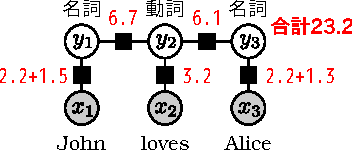
\includegraphics[height=10cm]{pos-tagging-score1.pdf}
      \end{beamercolorbox}
      \vskip\baselineskip
      \begin{beamercolorbox}{figure}
        \centering
        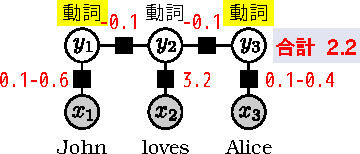
\includegraphics[height=10cm]{pos-tagging-score2.pdf}
      \end{beamercolorbox}
    \end{column}
    \begin{column}[t]{0.4\textwidth}\\
      \footnotesize
      \begin{table}
        \centering
        \begin{tabular}{l@{\hskip2em}r}
          \hline
          特徴 & 重み \\
          \hline
          $y_i = \text{名詞} \land \mathrm{CapInit}(x_i)$ & 2.2 \\
          $y_i = \text{動詞} \land \mathrm{CapInit}(x_i)$ & 0.1 \\
          $y_i = \text{名詞} \land x_i = \text{John}$ & 1.5 \\
          $y_i = \text{動詞} \land x_i = \text{John}$ & -0.6 \\
          $y_i = \text{名詞} \land x_i = \text{Alice}$ & 1.3 \\
          $y_i = \text{動詞} \land x_i = \text{Alice}$ & -0.4 \\
          $y_i = \text{名詞} \land x_i = \text{loves}$ & 0.1 \\
          $y_i = \text{動詞} \land x_i = \text{loves}$ & 3.2 \\
          \hline
          $y_i = \text{名詞} \land y_{i+1} = \text{名詞}$ & 1.3 \\
          $y_i = \text{動詞} \land y_{i+1} = \text{名詞}$ & 6.1 \\
          $y_i = \text{名詞} \land y_{i+1} = \text{動詞}$ & 6.7 \\
          $y_i = \text{動詞} \land y_{i+1} = \text{名詞}$ & -0.1 \\
          \hline
        \end{tabular}
        \caption{点数表}
      \end{table}
      \scriptsize
      ※ $\mathrm{CapInit}(x_i)$ は $x_i$ の先頭が大文字なら真
    \end{column}
  \end{columns}
\end{block}